\documentclass{article}
\usepackage[francais]{babel}
\usepackage[utf8]{inputenc}
\usepackage[T1]{fontenc}
\usepackage{lmodern}
\usepackage{amsmath}
\usepackage{amssymb}
\usepackage{mathrsfs}
\usepackage{tikz}
\usepackage{graphicx}
\usepackage{placeins}
\usepackage{listings}
\usepackage{cancel}
\usepackage{hyperref}
\usepackage{xcolor}
\usepackage{subcaption}
\colorlet{punct}{red!60!black}
\definecolor{background}{HTML}{EEEEEE}
\definecolor{delim}{RGB}{20,105,176}
\colorlet{numb}{magenta!60!black}
\lstdefinelanguage{json}{
    basicstyle=\normalfont\ttfamily,
    numbers=left,
    numberstyle=\scriptsize,
    stepnumber=1,
    numbersep=8pt,
    showstringspaces=false,
    breaklines=true,
    inputencoding=utf8,
    extendedchars=true,
    frame=lines,
    backgroundcolor=\color{background},
    literate=
        *{0}{{{\color{numb}0}}}{1}
        {1}{{{\color{numb}1}}}{1}
        {2}{{{\color{numb}2}}}{1}
        {3}{{{\color{numb}3}}}{1}
        {4}{{{\color{numb}4}}}{1}
        {5}{{{\color{numb}5}}}{1}
        {6}{{{\color{numb}6}}}{1}
        {7}{{{\color{numb}7}}}{1}
        {8}{{{\color{numb}8}}}{1}
        {9}{{{\color{numb}9}}}{1}
        {:}{{{\color{punct}{:}}}}{1}
        {,}{{{\color{punct}{,}}}}{1}
        {\{}{{{\color{delim}{\{}}}}{1}
        {\}}{{{\color{delim}{\}}}}}{1}
        {[}{{{\color{delim}{[}}}}{1}
        {]}{{{\color{delim}{]}}}}{1}
        {é}{{\'e}}{1}%
        {è}{{\`e}}{1}%
        {à}{{\`a}}{1}%
        {ç}{{\c{c}}}{1}%
        {œ}{{\oe}}{1}%
        {ù}{{\`u}}{1}%
        {É}{{\'E}}{1}%
        {È}{{\`E}}{1}%
        {À}{{\`A}}{1}%
        {Ç}{{\c{C}}}{1}%
        {Œ}{{\OE}}{1}%
        {Ê}{{\^E}}{1}%
        {ê}{{\^e}}{1}%
        {î}{{\^i}}{1}%
        {ô}{{\^o}}{1}%
        {û}{{\^u}}{1}%
        {ë}{{\¨{e}}}1
        {û}{{\^{u}}}1
        {â}{{\^{a}}}1
        {Â}{{\^{A}}}1
        {Î}{{\^{I}}}1,
}
\newcommand{\deriv}{\mathrm{d}}
\usepackage{array,multirow,makecell}
\usepackage[top=3cm, bottom=3cm, left=3cm,right=3cm]{geometry}
\usepackage{bbold}


\newtheorem{lemma}{Lemme}

\usepackage{fancyhdr}
\pagestyle{fancy}
\fancyhead[L]{M. \bsc{Augé} et M. \bsc{Roux}}
\fancyhead[C]{}
\fancyhead[R]{DistribEauPti - Rapport}
\renewcommand{\headrulewidth}{1pt}
\fancyfoot[C]{\thepage}

\newcolumntype{C}[1]{>{\centering\arraybackslash }b{#1}}
\setcounter{MaxMatrixCols}{20}
\renewcommand{\footrulewidth}{1pt}

\title{DistribEauPti \\ Rapport}
\date{\today}
\author{\bsc{Augé} Marc-Antoine et \bsc{Roux} Matthieu}

\begin{document}
\thispagestyle{empty}
\begin{center}

    \begin{figure}[!htb]
        \begin{center}
            
\includegraphics[width=4cm]{logoPonts.png}
        \end{center}
    \end{figure}
    
    \vspace{0.5cm}
    
    {\large{\bf École des Ponts ParisTech}}
    
    \vspace{0.2cm}
    
    {\large{\bf Mars 2018 - Avril 2018}}
    
    \vspace{1.5cm}
    
    \large{ \bf Cours Optimisation et Contrôle}\\
    \vspace{0.2cm}
    {\Large{\bf DistribEauPti - Projet sur les réseaux de distribution d'eau}}
    
    \vspace{1cm}
    
    \large{Marc-Antoine Augé et Matthieu Roux}

\end{center}
\newpage

\tableofcontents
 
\section{Séance 1 - Définition de l'oracle}
    \subsection{Calculs différentiels}
        On pose \[ F(q) = \frac{1}{3}<q, r \circ q \circ |q|> + <p_r, A_rq> \] et \[q(q_c) = q^{(0)} + Bq_c \]
        On cherche à calculer $\nabla F(q(q_c))$ et $H F(q(q_c))$ le Hessien.\\
        Remarquons tout d'abord que les matrices sont à coefficients réels donc transposition et adjonction sont deux opérations identiques.\\
        Commencons par $\nabla F(q)$ en écrivant le produit de Hadamard terme à terme et le produit scalaire sous forme de somme :
        \[ F(q) = \frac{1}{3}\sum_{i = 1}^n q_i^2.r_i.|q_i| + <p_r, A_rq>\]
        On note alors $\epsilon_i$ le signe de $q_i$ :
        \[ F(q) = \frac{1}{3}\sum_{i = 1}^n \epsilon_i.r_i.q_i^3 + <p_r, A_rq>\]
        D'où immédiatement, étant donné que le gradient du second terme est $A_r^T.p_r$ :
        \[\nabla F(q) = (\epsilon_i.r_i.q_i^2)_{1 \leq i \leq n} + A_r^T.p_r\]
        On peut le réécrire sans la notation $\epsilon_i$ et en utilisant un produit de Hadamard : 
        \[ \boxed{\nabla F(q) = (r_i.q_i.|q_i|)_{1 \leq i \leq n} + A_r^T.p_r
            = r\circ q \circ |q| + A_r^T.p_r}\]

        Puis par composition, comme $q(q_c) = q^{(0)} + q_c$, on a, en notant par abus de notation : $F(q_c) = F(q(q_c))$ :
        \[ \boxed{\nabla F(q_c) = B^T\nabla F(q) = B^T(r\circ q \circ |q| + A_r^T.p_r)  
        }\]

        Pour calculer le Hessien, on a tout d'abord, en notant $\text{diag}(X)$ la matrice diagonale possédant sur sa diagonale les coefficients de $X$ :
        \[H F(q) = 2.\text{diag}(r\circ|q|)\]
        Par composition, étant donné que le $H(q(q_c)) = 0$ :
        \[ \boxed{H F(q_c) = H F(q(q_c)) = 2.B^T.\text{diag}(r\circ|q|).B}
        \] 

    \paragraph{}

\section{Séances 2 et 3 - Implémentations d'algorithmes}

    Nous avons cherché à résoudre le problème d'optimisation avec différents algorithmes vus en cours :
    \begin{itemize}
        \item Mise en place d'une recherche linéaire vérifiant les conditions de Wolfe avec l'algorithme de Fletcher-Lemaréchal. Cette étape permet de trouver un pas optimal et conduit notamment à l'\textbf{algorithme de gradient à pas variable}.
        \item Mise en place de l'algorithme de \textbf{Polak-Ribière}, algorithme de gradient conjugué non-linéaire où la direction étudiée dépend de la direction de l'étape précédente.
        \item Mise en place de \textbf{l'algorithme de BFGS} (Broyden-Fletcher-Goldfarb-Shanno) qui est une méthode de quasi-Newton où on utilise une approximation de l'inverse du Hessien de la fonction à minimiser.
        \item Mise en place de \textbf{l'algorithme de Newton} qui n'approxime pas l'inverse du Hessien
    \end{itemize}

    \paragraph{}Nous avons obtenu les résultats présentés sur la Figure \ref{fig:courbes} et synthétisés sur le Tableau \ref{comparAlgo}. Nous remarquons notamment les points suivants :
    \begin{itemize}
        \item L'ajout de la recherche linéaire via l'algorithme de Fletcher-Lemaréchal est une très bonne amélioration qui demande un peu plus de calculs par itération mais en en faisant près de $10\times$ moins demeure deux fois plus rapide qu'un algorithme de gradient à pas fixe.
        \item L'algorithme de Newton est extrêmement rapide (6 itérations) mais demande une bonne connaissance du problème (le Hessien) : toutefois une approximation de ce Hessien, comme à travers l'algorithme BFGS donne également d'excellents résultats.
        \item L'initialisation dans l'algorithme de Fletcher-Lemaréchal est importante. Si on initialise avec le $\alpha$ précédent, comme sur la Figure \ref{fig:pas_variableAlpha}, alors la convergence est très mauvaise.
        \item On remarque que l'algorithme de Fletcher-Lemaréchal fait osciller le pas de gradient.
    \end{itemize}

    
    \begin{figure}
        \begin{subfigure}[t]{0.4\textwidth}
            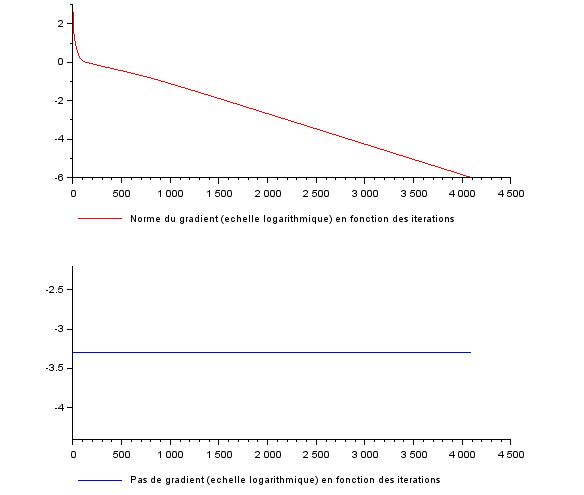
\includegraphics[width=\textwidth]{../Images/Pas_fixe.png}
            \label{fig:pas_fixe}
            \caption{Gradient à pas fixe}        
        \end{subfigure}
        \hfill
        \begin{subfigure}[t]{.4\textwidth}
            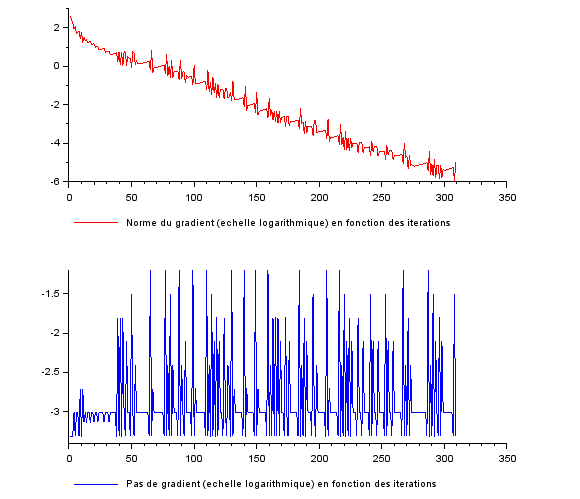
\includegraphics[width=\textwidth]{../Images/Pas_variable.png}
            \label{fig:pas_variable}
            \caption{Gradient à pas variable (conditions de Wolfe)}
        \end{subfigure}
        \hfill
        \begin{subfigure}[t]{.4\textwidth}
            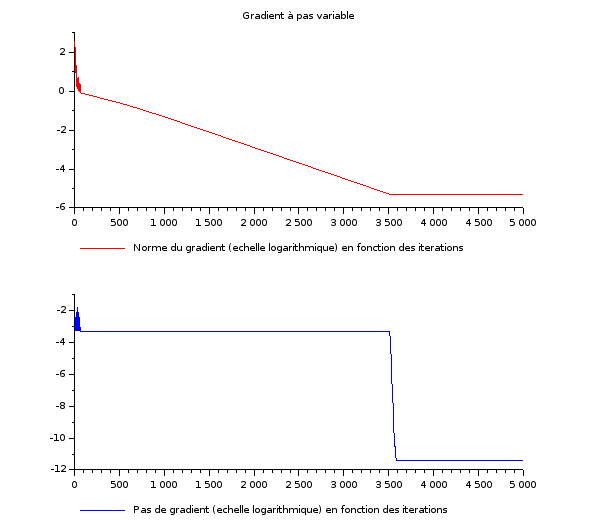
\includegraphics[width=\textwidth]{../Images/pas_variable_initAlpha.png}
            \label{fig:pas_variableAlpha}
            \caption{Gradient à pas variable où Fletcher-Lemaréchal initialité avec $\alpha$ précédent}
        \end{subfigure}
        \hfill
        \begin{subfigure}[t]{.4\textwidth}
            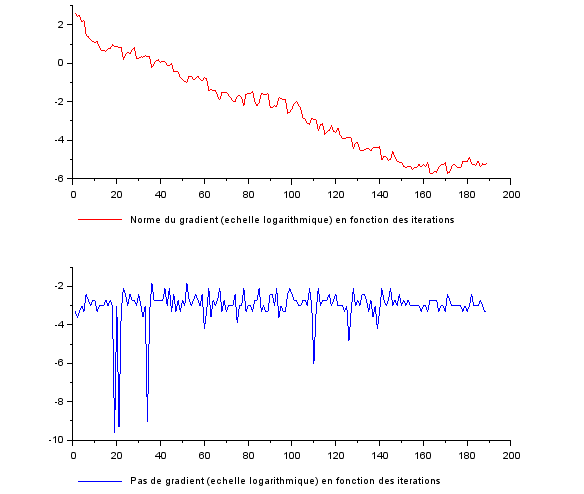
\includegraphics[width=\textwidth]{../Images/Polak_Ribiere.png}
            \label{fig:Polak_Ribiere}
            \caption{Polak-Ribière}
        \end{subfigure}
        \hfill
        \begin{subfigure}[t]{.4\textwidth}
            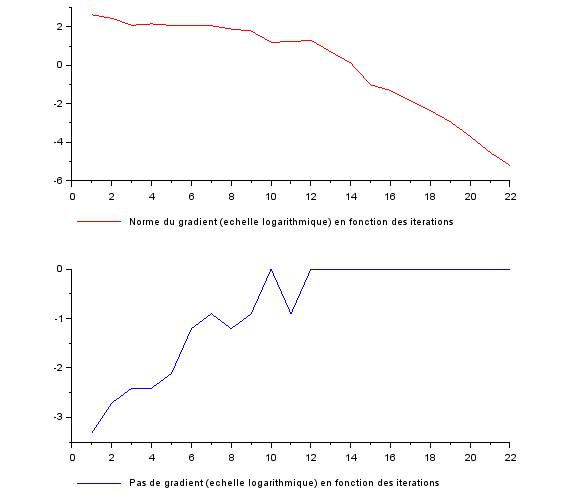
\includegraphics[width=\textwidth]{../Images/BFGS.png}
            \label{fig:BFGS}
            \caption{BFGS}
        \end{subfigure}
        \hfill
        \begin{subfigure}[t]{.4\textwidth}
            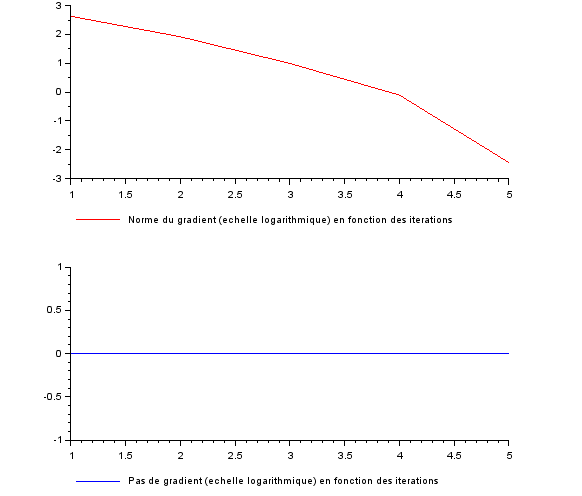
\includegraphics[width=\textwidth]{../Images/Newton.png}
            \label{fig:BFGS}
            \caption{Newton}
        \end{subfigure}
        \label{fig:courbes}
        \caption{Comparaison des différents algorithmes implémentés}
    \end{figure}
    \begin{figure}

        \begin{tabular}{|c|cccccc|}
            \hline
            Méthode & Scilab & Pas fixe & Pas variable & Polak-Ribiere & BFGS & Newton \\
            \hline 
            Itérations & - & 4094 & 310 & 190 & 23 & 6\\
            Temps CPU (s) & 0 & 0.34375 & 0.15625 & 0.109375 & 0.03125 & 0\\
            Critère optimal & -3.734007 & -3.734007 & -3.734007 & -3.734007 & -3.734007 & -3.734007\\
            Norme du gradient & $10^-7$ & $10^-6$ & $9.10^-7$ & $7.10^-7$ & $4.10^-7$ & $7.85.10^-8$\\
            \hline
        \end{tabular}
        \caption{Comparaison des différents algorithmes}
        \label{comparAlgo}
    \end{figure}

\end{document}

